\documentclass{article}
\input{../preamble}
\usepackage{cancel}
\input{unit2glossary}

\numberwithin{equation}{section}
\setcounter{section}{2}
\numberwithin{figure}{section}

\makeglossaries




\title{Unit 2: Constant Acceleration}
\author{Edited by Luis Nunez}
\date{Updated on \today}

\begin{document}

\maketitle

\subsection{Average Acceleration}

Recall that velocity is the speed and direction of an object. \Gls{acceleration} is the rate of change in velocity. It means speeding up or slowing down. 

\begin{mdframed}[backgroundcolor=black!10]
\Gls{average acceleration} is change in velocity divided by elapsed time.

\begin{equation}
    a = \frac{\Delta{v}}{\Delta{t}} = \frac{v_f - v_0}{t_f - t_0}
\end{equation}

\begin{center}
    \begin{tabular}{cl|cl}
    \hline
    \textbf{Symbol} & \textbf{Quantity} & \textbf{SI Base Unit} & \textbf{Unit Symbol}  \\
    \hline\hline
    \rule{0pt}{2.5ex}
        $a$ & average acceleration & meter per second squared & \SI{}{\meter/\second^2}\\
        $\Delta{v}$ & change in velocity & meter per second & m/s\\
        $\Delta{t}$ & elapsed time & second & s \\
    \hline
        $v_f$ & final velocity & meter per second & m/s\\
        $v_0$ & initial velocity & meter per second & m/s\\
        $t_f$ & final time & second & s \\    
        $t_0$ & initial time & second & s \\
        \hline
    \end{tabular}
\end{center}

Elapsed time is also known as \textit{change in time} or simply \textit{time}. Sometimes the $\Delta$ is dropped, and we symbolize elapsed time as just $t$, because it's typically assumed that initial time is $t_0 = 0$.
\end{mdframed}

\begin{example} \label{DcGEnk}
    Charlie drives hhis Porsche 911 at a constant velocity of \SI{45}{m/s} (\SI{101}{mph}) for 10 seconds. What is the average acceleration of the car?
\end{example}

\Solution Average acceleration is

\begin{equation*}
    a = \frac{\text{change in velocity}}{\text{change in time}} = 
    \frac{\Delta{v}}{\Delta{t}}
\end{equation*}

``Constant velocity'' means no change in velocity: 

\begin{equation*}
    \Delta{v} = \text{change in velocity} = \SI{0.0}{m/s}
\end{equation*}

Therefore,

\begin{equation*}
    a = \frac{\Delta{v}}{\Delta{t}} = \frac{0.0}{10.0} = \SI{0.0}{m/s^2}
\end{equation*}

\begin{example}
   Charlie's car goes from \SI{45}{m/s} to \SI{67}{m/s} (\SI{101}{mph} to \SI{150}{mph}) in \SI{4.3}{s}. What is his car's average acceleration? 
\end{example}

\Solution We are given the initial and final velocities and the elapsed time: $v_0 = \SI{45}{m/s}$, $v_f = \SI{67}{m/s}$, and $\Delta{t} = \SI{4.3}{s}$. The car's change in velocity is final velocity minus initial velocity:

\begin{equation*}
    \Delta{v} = v_f - v_0 = 67 - 45 = \SI{22}{m/s}
\end{equation*}

Therefore, it's average acceleration is


 \begin{equation*}
    a = \frac{\Delta{v}}{\Delta{t}} = \frac{22}{4.3} = \SI{5.1}{m/s^2}
\end{equation*}

\begin{exercise} \label{kVZPeG}
  Moby starts at rest and skates down a ramp to a velocity of \SI{15}{m/s} in 5.0 seconds. What is Moby's average acceleration? 
\end{exercise}

% \Solution To start from ``rest'' means that initial velocity is zero:

% \begin{equation*}
%     v_0 = \SI{0}{m/s}
% \end{equation*}

% Furthermore, we are given final velocity and elapsed time: $v_f = \SI{15}{m/s}$ and $\Delta{t} = \SI{5.0}{s}$. We want to find average acceleration: $a =\ ?$ The change in velocity is 

% \begin{equation*}
%     \Delta{v} = v_f - v_0 = \SI{15}{m/s} - 0 = \SI{15}{m/s}
% \end{equation*}

% Therefore, average acceleration is

% \begin{equation*}
%     \bar{a} = \frac{\Delta{v}}{\Delta{t}} = \frac{\SI{15}{m/s}}{\SI{5.0}{s}} = \SI{3.0}{m/s^2}\ 
% \end{equation*}

% An acceleration of \SI{3.0}{m/s^2} means with that every second that passes, Moby's velocity increases by \SI{3.0}{m/s}

% \framebox{\textbf{Link}} \textit{YouTube}: ``Acceleration -- Brain Pop'' by \texttt{Chase Harris} (\href{https://youtu.be/WmXnfHkPbYw}{click here}).

\begin{exercise} \label{Vth5N8}
    A subway train accelerates from rest to \SI{8.33}{m/s} in \SI{20.0}{s}. What is the average acceleration during that time interval?
\end{exercise}

\begin{exercise} \label{XSJU8b}
    Charles drives a car and accelerates from rest to \SI{12.8}{m/s} in \SI{17.0}{s}. What is the average acceleration during that time interval?
\end{exercise}


% \begin{choices}
% \choice \SI{12.8}{m/s}
% \choice \SI{2.70}{m/s^2}
% \choice \SI{45.9}{m/s^2}
% \CorrectChoice \SI{0.753}{m/s^2} 
% \end{choices}

%Relating the result of this problem (train's velocity at 17 s) to the previous counterpart created epiphanies for serveral students. When we showed that we arrive at the final velocity from the previous problem (12.8 m/s), some students went "Ohh, that's really cool!"

% \framebox{\textbf{Practice}} The same train departs from the station from rest and accelerates at \SI{0.753}{m/s^2}. Complete the table below, calculating changes in the train's velocity across time.

% \begin{figure}[h!]
%     \centering
%     \begin{tabular}{c|l}
%         \textbf{Time (s)} & \textbf{Velocity (m/s)} \\
%         \hline
%         0 & 0.000\\
%         1 & $0.000 + {\color{red}0.753}$\\
%         2 & $0.753 + {\color{red}0.753} = 1.506$ \\
%         3 & $1.506 + {\color{red}0.753} = 2.259$ \\
%         4 & $2.259 + {\color{red}0.753} = 3.012$ \\
%         \vdots &  \\
%         17 &  \\
%     \end{tabular}
% \end{figure}


\begin{example}
    A golf ball rolls at \SI{2.7}{m/s} near the top of an inclined ramp. When it starts rolling down the ramp, it accelerates at \SI{4.9}{m/s^2} for \SI{5.0}{s}. What is the golf ball's final velocity?
\end{example}

\Solution We are given the ball's initial velocity, acceleration, and time:

\begin{equation*}
    v_0 = \SI{2.7}{m/s}, \quad
    a = \SI{4.9}{m/s^2}, \quad
    \Delta{t} = \SI{5.0}{s}
\end{equation*}

We want to find the final velocity: $v_f =\ ?$. These quantities are related by the equation for average acceleration:

\begin{equation*}
    a = \frac{v_f - v_0}{\Delta{t}}
\end{equation*}

Substituting numbers leads to

\begin{equation*}
    4.9 = \frac{v_f - 2.7}{5.0}\ ,
\end{equation*}

This equation is solved for final velocity ($v_f$) as follows:

\begin{align*}
    \hspace{-10em} \textbf{Put $v_f$ on left} \hspace{5em} & \frac{v_f - 2.7}{5.0} = 4.9\\[1ex]
   \hspace{-10em} \textbf{Multiply by 5.0} \hspace{5em} & \frac{v_f - 2.7}{\cancel{5.0}} \mathbin{\color{red}\times} \textcolor{red}{\cancel{5.0}} = 4.9 \mathbin{\color{red}\times} \textcolor{red}{5.0}\\[1ex] 
   \hspace{-10em} \textbf{Simplify} \hspace{5em} & v_f - 2.7 = 24.5\\[1ex]
   \hspace{-10em} \textbf{Add 2.7} \hspace{5em} & v_f - 2.7 \mathbin{\color{red} +} \textcolor{red}{2.7} = 24.5 \mathbin{\color{red} +} \textcolor{red}{2.7}\\[1ex]
   \hspace{-10em} \textbf{Simplify} \hspace{5em} & v_f = 27.2\\
\end{align*}

Therefore the final velocity of the golf ball is \SI{27.2}{m/s}.

\begin{example}
  A vehicle accelerates a at \SI{2.47}{m/s^2}. How much time (in seconds) does it take this car to change its speed from \SI{18}{m/s} to \SI{25}{m/s}?  
\end{example}

\Solution We are given acceleration and initial and final velocities:

\begin{equation*}
    a = \SI{2.47}{m/s^2}\ , \quad
    v_0 = \SI{18}{m/s}\ , \quad
    v_f = \SI{25}{m/s}
\end{equation*}

We want to find the elapsed time, $\Delta{t}$. These quantities are related by the average acceleration equation:

\begin{equation*}
    a = \frac{v_f - v_0}{\Delta t}
\end{equation*}

Substituting the known values into this equation leads to

\begin{equation*}
    2.47 = \frac{25 - 18}{\Delta t}\ ,
\end{equation*}

which is

\begin{equation*}
    2.47 = \frac{7}{\Delta t}
\end{equation*}

We may solve this equation for elapsed time ($\Delta t$) as follows:

\begin{align*}
    \hspace{-10em} \textbf{Multiply by $\Delta t$} \hspace{5em} & 2.47 \cdot \textcolor{red}{\Delta t} =  \frac{7}{\cancel{\Delta t}} \cdot \textcolor{red}{\cancel{\Delta t}}\\[1ex]
    \hspace{-10em} \textbf{Simplify} \hspace{5em} & 2.47 \cdot \Delta t = 7\\[1ex]
    \hspace{-10em} \textbf{Divide by 2.47} \hspace{5em} & \frac{\cancel{2.47} \cdot \Delta t}{\textcolor{red}{\cancel{2.47}}} = \frac{7}{\textcolor{red}{2.47}}\\[1ex]
    \hspace{-10em} \textbf{Simplify} \hspace{5em} & t = \SI{2.83}{s}
\end{align*}

Therefore, it takes this vehicle \SI{2.83}{s} to change speed.


\subsection{Velocity vs.~Time Graphs}

\begin{mdframed}[backgroundcolor=black!10]
    In a velocity vs.~time graph, displacement is the area under the curve.
\end{mdframed}



\begin{example}
The velocity-time graph shows the motion of an accelerating object. What is the object's displacement throughout the entire time interval?
\end{example}

\begin{center}
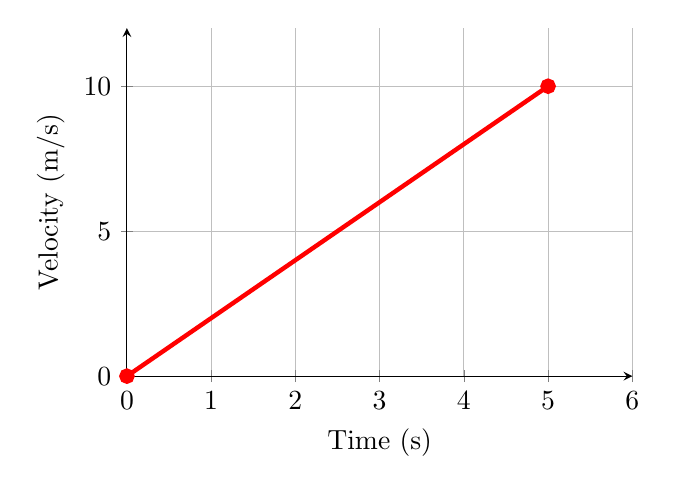
\begin{tikzpicture}
\begin{axis}[width=8cm, height=6cm,
        axis lines=left,
        ymin=0, ymax=12,
        xmin=0, xmax=6,
        ylabel = Velocity (m/s),
        xlabel = Time (s),
        grid=both,
        ytick={0,5,...,15},
    ]
    \addplot[
        color=red,
        mark options={color=red},mark=*,
        ultra thick,
        ]
        coordinates {
        (0,0)(5,10)
        };
\end{axis}
\end{tikzpicture}
\end{center}

\Solution Displacement is the area under the curve. The bounded area is a right triangle, whose area is given by its base ($b$) multiplied by its height ($h$), divided by 2:

\begin{equation*}
    A = \frac{b h}{2}\ .
\end{equation*}

\begin{center}
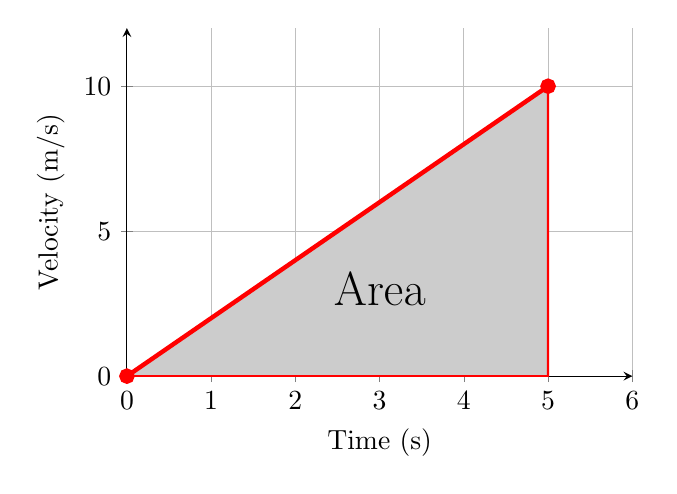
\begin{tikzpicture}
\begin{axis}[width=8cm, height=6cm,
        axis lines=left,
        ymin=0, ymax=12,
        xmin=0, xmax=6,
        ylabel = Velocity (m/s),
        xlabel = Time (s),
        grid=both,
        ytick={0,5,...,15},
    ]
    \draw[red,thick,fill=black!20] (axis cs: 0,0) -- (axis cs: 5,10) -- (axis cs: 5,0) -- (axis cs: 0,0);
    \addplot[
        color=red,
        mark options={color=red},mark=*,
        ultra thick,
        ]
        coordinates {
        (0,0)(5,10)
        };
    \node at (axis cs: 3,3) {\LARGE Area};
\end{axis}
\end{tikzpicture}
\end{center}

The base is 5, the height is 10, so the triangle's area is

\begin{equation*}
    A = \frac{bh}{2} = \frac{5 \times 10}{2} = 25
\end{equation*}

Therefore, the object's displacement is \SI{25}{m}.

\begin{example}
The graph represents an object's motion. What is the displacement of the object throughout the entire time interval?
\end{example}

\begin{center}
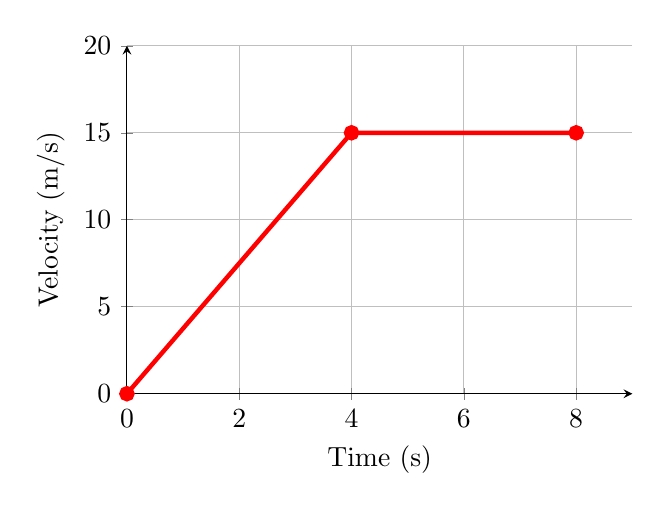
\begin{tikzpicture}
\begin{axis}[width=8cm, height=6cm,
        axis lines=left,
        ymin=0, ymax=20,
        xmin=0, xmax=9,
        ylabel = Velocity (m/s),
        xlabel = Time (s),
        grid=both,
        ytick={0,5,...,20},
    ]
    \addplot[
        color=red,
        mark options={color=red},mark=*,
        ultra thick,
        ]
        coordinates {
        (0,0)(4,15)(8,15)
        };
\end{axis}
\end{tikzpicture}
\end{center}

\Solution Displacement is the area under the curve. Two regions are bounded by the curve: a triangle ($A=bh/2$) and a rectangle ($A = lw$).

\begin{center}
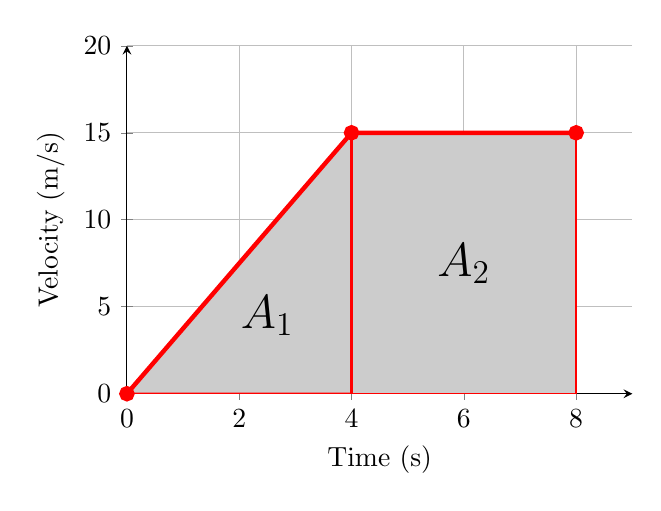
\begin{tikzpicture}
\begin{axis}[width=8cm, height=6cm,
        axis lines=left,
        ymin=0, ymax=20,
        xmin=0, xmax=9,
        ylabel = Velocity (m/s),
        xlabel = Time (s),
        grid=both,
        ytick={0,5,...,20},
    ]
    \draw[red,thick,fill=black!20] (axis cs: 0,0) -- (axis cs: 4,15) -- (axis cs: 4,0) -- (axis cs: 0,0);
    \draw[red,thick,fill=black!20] (axis cs: 4,0) rectangle (axis cs: 8,15);
    \node at (axis cs: 2.5,4.5) {\LARGE $A_1$};
    \node at (axis cs: 6,7.5) {\LARGE $A_2$};
    \addplot[
        color=red,
        mark options={color=red},mark=*,
        ultra thick,
        ]
        coordinates {
        (0,0)(4,15)(8,15)
        };
\end{axis}
\end{tikzpicture}
\end{center}

% \begin{figure}[h!]
%     \centering
% \begin{tikzpicture}
% \begin{axis}[width=300pt, height=207pt,
%         axis y line=left, 
%         axis x line=left,
%         ymin=0, ymax=20,
%         xmin=0, xmax=9,
%         ylabel = Velocity (m/s),
%         xlabel = Time (s),
%         grid=both,
%         ytick={0,5,...,20},
%         yminorgrids=true, minor y tick num=4,
%         xminorgrids=true, minor x tick num=4,
%     ]
%     \draw[red,thick,fill=black!20] (axis cs: 0,0) -- (axis cs: 4,15) -- (axis cs: 4,0) -- (axis cs: 0,0);
%     \draw[red,thick,fill=black!20] (axis cs: 4,0) rectangle (axis cs: 8,15);
%     \node at (axis cs: 2.5,4.5) {\LARGE $A_1$};
%     \node at (axis cs: 6,7.5) {\LARGE $A_2$};
%     \addplot[
%         color=red,
%         mark options={color=red},mark=*,
%         ultra thick,
%         ]
%         coordinates {
%         (0,0)(4,15)(8,15)
%         };
% \end{axis}
% \end{tikzpicture}
% \end{figure}

The areas of the triangle and rectangle, respectively, are
\vspace{-1em}

\begin{align*}
    A_1 &= \frac{bh}{2} = \frac{4 \times 15}{2} = 30\\[1ex]
    A_2 &= lw = 4 \times 15 = 60
\end{align*}

The total area (and, therefore, total displacement) is the sum of the two areas:

\begin{equation*}
    A = A_1 + A_2 = 30 + 60 = 90
\end{equation*}

Therefore, the total displacement is $+\SI{90}{m}$.

\begin{example}
An object travels in one direction at a constant velocity, then instantaneously changes direction to a slower speed. Calculate the object's displacement throughout the entire time interval.
\end{example}

\begin{center}
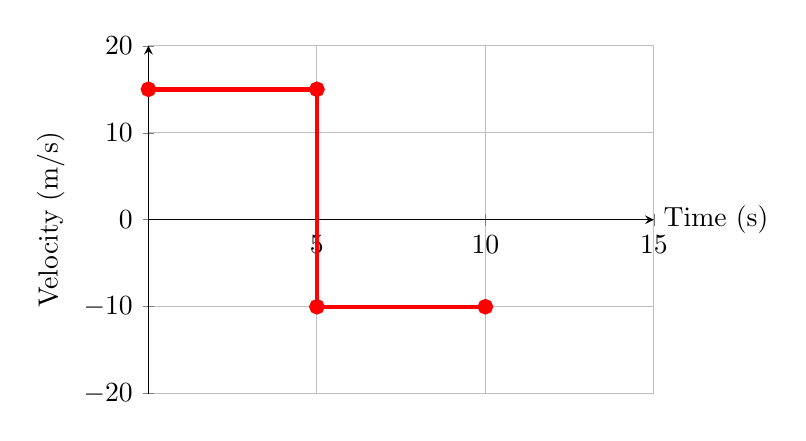
\begin{tikzpicture}
\begin{axis}[width=8cm,height=6cm,
    axis y line=left, 
    axis x line=center,
    xlabel = Time (s),
    ylabel = Velocity (m/s),
    ymin=-20, ymax=20,
    xmin=0, xmax=15,
    ytick={-20,-10,...,20},
    xtick={0,5,...,15},
    grid=both,
    x label style={anchor=west},
    clip=false,
]
    \addplot[
        color=red,
        mark options={color=red},mark=*,
        ultra thick,
        ]
        coordinates {
        (0,15)
        (5,15)
        (5,-10)
        (10,-10)
        };
\end{axis}
\end{tikzpicture}
\end{center}

\Solution Displacement is the area under the curve. The regions bounded by the curve are two rectangles:

\begin{center}
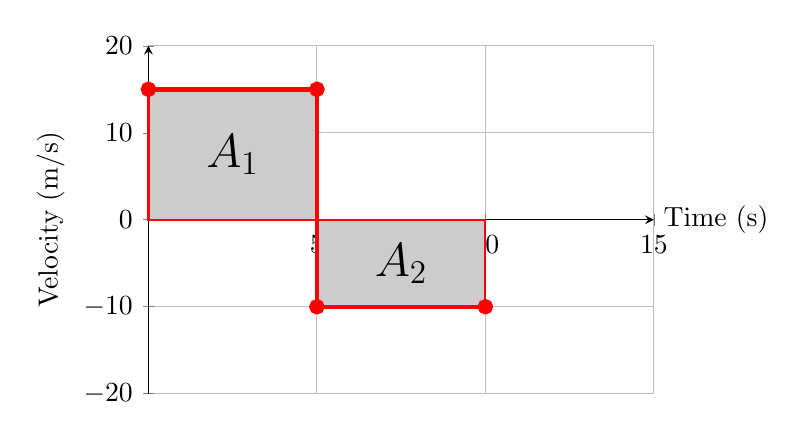
\begin{tikzpicture}
\begin{axis}[width=8cm,height=6cm,
    axis y line=left, 
    axis x line=center,
    xlabel = Time (s),
    ylabel = Velocity (m/s),
    ymin=-20, ymax=20,
    xmin=0, xmax=15,
    ytick={-20,-10,...,20},
    xtick={0,5,...,15},
    grid=both,
    x label style={anchor=west},
    clip=false,
]
    \draw[red,thick,fill=black!20] (axis cs: 0,0) rectangle (axis cs: 5,15);
    \draw[red,thick,fill=black!20] (axis cs: 5,-10) rectangle (axis cs: 10,0);
    \node at (axis cs: 2.5,7.5) {\LARGE $A_1$};
    \node at (axis cs: 7.5,-5) {\LARGE $A_2$};
    \addplot[
        color=red,
        mark options={color=red},mark=*,
        ultra thick,
        ]
        coordinates {
        (0,15)
        (5,15)
        (5,-10)
        (10,-10)
        };
\end{axis}
\end{tikzpicture}
\end{center}

Recall that for a rectangle, $\text{area} = \text{length} \times \text{width}$. The areas of the rectangles are
\vspace{-1em}

\begin{align*}
    A_1 &= 5 \times 15 = 75\\[1ex]
    A_2 &= 5 \times (-10) = -50
\end{align*}

$A_2$ being negative represents a \textit{negative} displacement, as the object's velocity is negative in this region. The total area (and, therefore, total displacement) is the sum of two areas:

\begin{equation*}
    A = A_1 + A_2 = 75 + (-50) = +25
\end{equation*}

Therefore, total displacement is $+\SI{25}{m}$.

\vspace{2ex}

\cyanhrule


\subsection{Answers to Select Exercises}

\ref{kVZPeG}. \SI{3.0}{m/s^2}\\
\ref{Vth5N8}. \SI{0.417}{m/s^2}\\
\ref{XSJU8b}. \SI{0.753}{m/s^2}\\
% \ref{DcGEnk}. \SI{0.0}{m/s^2}



\end{document}

% \textit{YouTube}: ``Shuttle Launch'' (\href{https://youtu.be/uuYoYl5kyVE}{link})

% How does acceleration play a role in the launching of a space shuttle? Think about initial and final velocities and the time interval of the launch.\\


% \textit{YouTube}: ``Position, Velocity, Acceleration'' by Professor Dave Explains (\href{https://youtu.be/4dCrkp8qgLU?t=260}{link})

% \textit{YouTube}: ``Spider-Man Stops a Train from Crashing'' by Voyage (\href{https://youtu.be/r_W6mXqzJNU?t=260}{link})


% \textit{YouTube}: ``Acceleration'' by Khan Academy (\href{https://youtu.be/FOkQszg1-j8}{link})



% \textit{Physics Classroom} Concept Builder: Name That Motion (\href{https://www.physicsclassroom.com/Concept-Builders/Kinematics/Name-That-Motion/Concept-Builder}{link})

% \hrule

% \textit{Physics Classroom} Concept Builder: Acceleration (\href{https://www.physicsclassroom.com/Concept-Builders/Kinematics/Acceleration/Concept-Builder}{link})



% \framebox{\textbf{Link}} \textit{YouTube}: ``Solving Average Acceleration Example 1'' by \texttt{Calebrese Physics} (\href{https://youtu.be/uA42ScL_gHI}{click here})

% \subsection{Velocity vs.~Time Graphs}

% \begin{figure}[h!]
%     \centering
%     \scalebox{0.9}{
%     \begin{tikzpicture}
%     \begin{axis}[axis y line=left, 
%         axis x line=left,
%         ymin=0, ymax=70,
%         xmin=0, xmax=35,
%         ylabel = Velocity (m/s),
%         xlabel = Time (s),
%         grid=both,
%         ytick={0,10,...,70},
%         xtick={0,5,...,35}
%     ]
%     \addplot[
%         %color=green!67!black,
%         color=black,
%         mark options={color=black},mark=none,
%         ultra thick,
%         ]
%         coordinates {
%         (0,0)(30,60)
%         };
%     \end{axis}
%     \end{tikzpicture}
%     }
%     \caption{Caption}
%     \label{fig:Ch2_Prob51}
% \end{figure}


% \begin{tabular}{|p{2in}|p{3in}|c|}
%     \hline
%     \textbf{Problem Set} & \textbf{Learning Objective} & \textbf{Due Date} \\
%     \hline
%      K6: Acceleration 1 & Use the $\bar{a} = \Delta v/\Delta t$ equation to solve straight-forward problems involving a calculation of acceleration. & \\
%      \hline
%      K7: Acceleration 2 & Use the $\bar{a} = \Delta v/\Delta t$ equation to solve less-than-routine problems & \\
%      \hline
%      K10: Velocity-Time Graphs 1 & Use a velocity-time graph to determine an object's acceleration at indicated times. & \\
%      \hline
%      K11: Velocity-Time Graphs 2 & Use a velocity-time graph to determine an object's displacement at indicated times and during indicated time periods. & \\
%      \hline
% \end{tabular}


% \textit{Physics Classroom} Concept Builder: Motion Diagrams (\href{https://www.physicsclassroom.com/Concept-Builders/Kinematics/Motion-Diagrams/Interactive}{link})

% \textit{Physics Classroom} Concept Builder: Graph That Motion (\href{https://www.physicsclassroom.com/Concept-Builders/Kinematics/Graph-That-Motion/Concept-Builder}{link})



% \section*{Understanding the Four Forces}

% \colorbox{yellow}{\textbf{force}} a push or pull on an object

% Gravity is one of the 4 fundamental forces.

% Gravity explains why a dropped ball falls to the ground. It also explains why our planet orbits the Sun. 

% Gravity from Earth pushes you and all objects towards the ground.

% % \textit{YouTube}: ``The Four Fundamental Forces of nature'' (\href{https://youtu.be/669QUJrF4u0}{link})




% % \begin{figure}[h!]
% %     \centering
% %     \begin{tabular}{l|c|l}
% %         \hline
% %         \textbf{Force} & \textbf{Approximate Relative Strength} & \textbf{Range}  \\
% %         \hline \hline
% %         Gravity & \SI{e-38}{} & $\infty$ \\
% %         Weak & \SI{e-13}{} & $< \SI{e-18}{\meter}$ \\
% %         Electromagnetic & \SI{e-2}{} & $\infty$ \\
% %         Strong & 1 & $< \SI{e-15}{\meter}$ \\
% %         \hline
% %     \end{tabular}
% %     \caption{Relative strength and range of the four fundamental forces. Relative strength is based on the strong force felt by a proton–proton pair.}
% %     \label{fig:Table_FourFundForces}
% % \end{figure}

% \section*{Concepts Related to Newton’s Law of Universal Gravitation}


% Isaac Newton was the first to define the gravitational force.

% Gravitational force is always attractive. It depends only on the masses involved and the distance between them. 

% \textit{PhET Simulations}: Gravity Force Lab (\href{https://phet.colorado.edu/sims/html/gravity-force-lab/latest/gravity-force-lab_en.html}{link})

% \colorbox{yellow}{\textbf{Newton’s universal law of gravitation}} states that the gravitational force between two objects is directly proportional to the product of their masses and inversely proportional to the square of the distance between them.

% \begin{equation}
%     F = \frac{G m M}{r^2}
% \end{equation}

% \begin{figure}[h!]
%     \centering
%     \begin{tabular}{cl|cc}
%     \hline
%     \textbf{Symbol} & \textbf{Quantity} & \textbf{SI Unit} & \textbf{Symbol}  \\
%     \hline\hline
%         $F$ & gravitational force & newton & N\\
%         $m$ & mass 1 & kilogram & kg \\
%         $M$ & mass 2 & kilogram & kg \\
%         $r$ & separation distance & meter & m \\
%     \hline
%     \end{tabular}
%     \label{tab:Gravitation}
% \end{figure}

% \begin{figure}[h!]
% \centering
%     \begin{tabular}{clll}
%     \hline
%     \textbf{Constant Symbol} & \textbf{Constant meaning} & \textbf{Value} & \textbf{Units} \\
%     \hline
%     $G$ & gravitational constant & \SI{6.673e-11}{} & \SI[per-mode=fraction]{}{{\newton\cdot\meter^2}\per{\kilogram^2}}\\
%     \hline
%     \end{tabular}
% \end{figure}


% \textit{PhET Simulation}: Gravity and Orbits (\href{https://phet.colorado.edu/sims/html/gravity-and-orbits/latest/gravity-and-orbits_en.html}{link})

% \colorbox{yellow}{\textbf{gravitational constant ($G$)}} the proportionality constant in Newton’s law of universal gravitation


% $G$ determines the strength of gravity, one of the four forces in nature.

% $G$ was determined experimentally in 1798 by Henry Cavendish.

% \vspace{1em} \hrule

% \textit{YouTube}: Gravitational Attraction (\href{https://youtu.be/Ym6nlwvQZnE}{link})

% \textit{YouTube}: The Cavendish Experiment (\href{https://youtu.be/2PdiUoKa9Nw}{link})

% \vspace{1em} \hrule

% \section*{Calculations Based on Newton’s Law of Universal Gravitation}

% % \begin{figure}[h!]
% %     \centering
% %     \includegraphics[width=0.5\textwidth]{Figures/Unit07_Fig7.8.jpg}
% %     \caption{Caption}
% %     \label{fig:Unit07_Fig7.8}
% % \end{figure}

% Mass and weight are NOT the same thing.

% \colorbox{yellow}{\textbf{mass}} the amount of matter in an object

% \colorbox{yellow}{\textbf{weight}} the force of gravity on an object

% The mass ($m$) of an object does not change.

% Weight changes depending on the gravitational field ($g$) of a planet or moon. For example, your weight on the Moon is less than your weight on Earth.

% The gravitational field ($g$) is an acceleration. 

% The relationship between force, mass, and acceleration from the second law of motion can be written in terms of $g$.

% \begin{equation*}
%     F = ma = mg
% \end{equation*}

% The force is the weight of the object, which is caused by the gravitational attraction of the planet or moon on which the object is located.





% % \begin{equation*}
% %     g = \frac{G M}{r^2}
% % \end{equation*}


% \colorbox{green}{\textbf{We do}} \textit{YouTube}: ``Mass and weight clarification'' by Khan Academy (\href{https://youtu.be/IuBoeDihLUc}{link})

% \colorbox{cyan}{\textbf{You do}} \textit{OpenStax}: Grasp Check: Would you have the same mass on the moon as you do on Earth? Would you have the same weight? (\href{https://openstax.org/books/physics/pages/7-2-newtons-law-of-universal-gravitation-and-einsteins-theory-of-general-relativity}{link})

% Introduction to Newton's Law of Gravitation 

% \colorbox{green}{\textbf{We do}} \textit{OpenStax}: Grasp Check: What is the difference between $g$ and $G$? (\href{https://openstax.org/books/physics/pages/7-2-newtons-law-of-universal-gravitation-and-einsteins-theory-of-general-relativity}{link})

% \colorbox{green}{\textbf{We do}} \textit{OpenStax}: Worked Example: Change in $g$ (\href{https://openstax.org/books/physics/pages/7-2-newtons-law-of-universal-gravitation-and-einsteins-theory-of-general-relativity}{link})

% \colorbox{green}{\textbf{We do}} \textit{OpenStax}: Worked Example: Earth's $g$ at the Moon (\href{https://openstax.org/books/physics/pages/7-2-newtons-law-of-universal-gravitation-and-einsteins-theory-of-general-relativity}{link})

% \colorbox{green}{\textbf{We do}} \textit{YouTube}: ``Factor of Change Method`` by Brentwood Christian School (\href{https://youtu.be/N65mxpBT-ts}{link})

% \colorbox{cyan}{\textbf{You do}} \textit{OpenStax}: Practice Problems \#6, 7 (\href{https://openstax.org/books/physics/pages/7-2-newtons-law-of-universal-gravitation-and-einsteins-theory-of-general-relativity}{link})

% \colorbox{cyan}{\textbf{You do}} \textit{OpenStax}: Check Your Understanding \#8, 9, 10 (\href{https://openstax.org/books/physics/pages/7-2-newtons-law-of-universal-gravitation-and-einsteins-theory-of-general-relativity}{link})

\begin{enumerate}
\setlength\itemsep{0.1ex}
    \item \label{goal:Calc_DeltaV} Calculate change in velocity given initial and final velocities
    \item Calculate acceleration of an object starting from rest given final velocity and time
    \item Calculate acceleration given initial velocity, final velocity, and time
    \item \label{goal:Solve_AccelEq_FinalVel}  Use the $a = \Delta{v}/\Delta{t}$ equation to solve for final velocity given initial velocity, acceleration, and time
    \item \label{goal:Solve_AccelEq_Time} Use the $a = \Delta{v}/\Delta{t}$ equation to solve for time given initial velocity, final velocity, and acceleration.
    \item Understand the relation between displacement and area bounded by a curve in a velocity vs.~time graph
    \item Calculate displacement in a velocity vs.~time graph for a region of constant velocity.
    \item Calculate displacement in a velocity vs.~time graph for a region of constant acceleration.
\end{enumerate}

\begin{center}
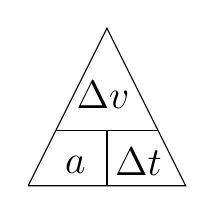
\begin{tikzpicture}
\draw (0,0) -- (2,0) -- (1,2) -- (0,0);
\node[anchor=north] at (0.6,0.5) {\Large $a$};
\node[anchor=north] at (1.4, 0.6) {\Large $\Delta{t}$};
\node[anchor=north] at (0.95,1.45) {\Large $\Delta{v}$};
\draw (0.35,0.7) -- (1.65,0.7);
\draw (1,0.7) -- (1,0);
\end{tikzpicture}
\end{center}